\documentclass[article]{jss}
\usepackage{thumbpdf,lmodern}
\usepackage[utf8]{inputenc}
\usepackage[margin=1.25in]{geometry}
\usepackage{amsmath}
\usepackage{amssymb}
\usepackage{graphicx}
\usepackage{dsfont}
\usepackage{tikz}
\usepackage{algorithm}
\usepackage{algorithmic}
\usepackage{eqparbox}
%% new custom commands
\newcommand{\class}[1]{`\code{#1}'}
\newcommand{\fct}[1]{\code{#1()}}

%% For Sweave-based articles about R packages:
%% need no \usepackage{Sweave}

\raggedbottom
\graphicspath{ {./images/} }
\renewcommand{\algorithmiccomment}[1]{\hfill\eqparbox{COMMENT}{\# #1}}
\makeatletter
\newcommand{\distas}[1]{\mathbin{\overset{#1}{\kern\z@\sim}}}%
\newsavebox{\mybox}\newsavebox{\mysim}
\newcommand{\distras}[1]{%
  \savebox{\mybox}{\hbox{\kern3pt$\scriptstyle#1$\kern3pt}}%
  \savebox{\mysim}{\hbox{$\sim$}}%
  \mathbin{\overset{#1}{\kern\z@\resizebox{\wd\mybox}{\ht\mysim}{$\sim$}}}%
}
\makeatother



\author{Eric Weine\\University of Chicago
   \And Mary Sara McPeek\\University of Chicago}
\Plainauthor{Eric Weine, Mary Sara McPeek}

\title{Efficient Calculation of Improved Simultaneous Testing Bands for QQplots}
%\author{Eric Weine and Mary Sara McPeek}
\Abstract{
Quantile-Quantile plots (QQplots) are often difficult to interpret because it is unclear how large the deviation from the theoretical distribution must be to indicate a lack of fit. Current packages and algorithms towards this end either do not ensure a robust Type I error rate, are too slow, or are under-powered to deviations in the tails of the distribution. In this paper, we present an efficient algorithm that computes simultaneous testing bands for QQplots. These bands have a variety of desirable properties, including being fast to compute and being equally sensitive to deviations in all parts of the null distribution, including the tails.
}

\Keywords{QQplots, Equal Local Levels, Kolmolgorov-Smirnov, GWAS, Multiple Testing}

\Address{
  Mary Sara McPeek\\
  Department of Statistics\\
  University of Chicago\\
  924 E 57th St., Chicago, IL\\
  E-mail: \email{mcpeek@uchicago.edu}\\
  URL: \url{https://galton.uchicago.edu/~mcpeek/}
}
\begin{document}

\maketitle

\section{Introduction}
Quantile-Quantile plots (QQplots) are a common statistical tool used to judge if a sample comes from a specified distribution \citep{wilk_gnanadesikan_1968}. Despite their ubiquity, they are often difficult to interpret because it is challenging to determine if the magnitude of the deviation from the specified distribution is large enough to indicate a lack of fit as opposed to sampling variance. To make this determination, it is useful to put testing bands on a QQplot.
\newline
\newline
A number of methods have been created towards this end. First, some available software puts pointwise testing bands onto QQplots, which conduct $\alpha$ level tests on each order statistic \citep{qqplotr}. This method is clearly insufficient, as it ignores the multiple testing problem and thus provides no guarantee on the Type I error rate of testing the global null hypothesis that all of the data come from the specified distribution. Second, the Komolgorov-Smirnov (KS) test is a common method for creating joint bands \citep{kolmogoroff1941confidence, smirnov1944approximate}. While this method ensures the correct Type I error by using the distribution of the KS statistic, this test suffers from very low power under a variety of reasonable alternatives \citep{aldor2013power}. In the same work, Aldor-Noiman et al. introduced a much more powerful test (under most alternatives) called the Tail Sensitive (TS) test. This test uses simulation to conduct an $\eta$ level test on each order statistic such that the overall test has an $\alpha$ level Type I error. This test has a variety of desirable properties, but because it requires simulation it is extremely slow in large datasets.
\newline
\newline
In what follows, we present a method that yields the same results as the TS test but does so substantially faster because of an efficient recursive calculation. We then demonstrate this test on a few multiple testing scenarios including Type I error calibration and genetic studies.
\section{Methods}

\subsection{Local Levels For Global Null Hypothesis Testing}

Suppose we have observations

\begin{equation*}
  X_{1}, ..., X_{n} \distras{iid} F,
\end{equation*}
and we are interested in conducting the following hypothesis test

\begin{equation*}
      H_{0}: F = F_{0} \textrm{ vs. } H_{A}: F \neq F_{0}
\end{equation*}
with level $\alpha$, where all parameters of $F_{0}$ are known. One approach to this problem, referred to as ``local levels,'' is to conduct separate hypothesis tests on each of the order statistics $X_{(i)}$, where each test has Type I error rate $\eta_{i}$ \citep{gontscharuk2016goodness}. Then, we reject the global null hypothesis if at least one of the $n$ tests results in a rejection. That is, we construct a set of intervals

\begin{equation*}
    (h_{1}, g_{1}), ..., (h_{n}, g_{n}),
\end{equation*}
and we reject $H_{0}$ if for any $i$

\begin{equation*}
    X_{(i)} \not\in (h_{i}, g_{i}).
\end{equation*}
If we know the local level $\eta_{i}$, then
\begin{equation}
    h_{i} = F^{-1}_{i}(\eta_{i} / 2) \text{ and } g_{i} = F^{-1}_{i}(1 - \eta_{i} / 2),
\end{equation}
where $F_{i}$ is the CDF of the $i^{th}$ order statistic. Thus, the difficulty is in determining an appropriate vector of local levels $(\eta_{1}, ..., \eta_{n})$ for which the resulting global level is $\alpha$. In our case, we want to create testing bands that are ``agnostic'' to any alternative distribution. By this, we mean that we would like to design a test that applies equal scrutiny to each order statistic, and thus we set
% an alternative explanation is that we're trying to design a test that would have optimum power under the alternative distribution where the probability of any of the order statistics being outside of the pointwise null region is equal.
\begin{equation}
    \eta_{1} = \eta_{2} = ... = \eta_{n} = \eta.
\end{equation}

This is known as ``equal local levels.''
\newline
\newline
\noindent Given the sample size $n$ and the desired level $\alpha$ we present the following algorithm for obtaining $\eta$ in two steps:
\newline
\newline
1. Given a proposed testing region $(h_{1}, g_{1}), ..., (h_{n}, g_{n})$, where $h_{i} < g_{i}$ for $i = 1, ..., n$, find the probability of $X_{(1)}, ..., X_{(n)}$ falling outside of this region under the null.
\newline
\newline
2. Using the algorithm described in step 1, conduct a binary search on the space of the local level $\eta$. This involves proposing a value of $\eta$, calculating the corresponding region $(h_{1}, g_{1}), ..., (h_{n}, g_{n})$ using equation (1), and then using step 1 to check if the region achieves the desired global Type I error rate $\alpha$.
\newline
\newline
We now describe these two steps in more detail:
\newline
\newline
\textbf{Step 1:} First, note that under the null hypothesis,

\begin{equation*}
    F_{0}(X_{1}), ..., F_{0}(X_{n}) \distras{iid} U(0, 1).
\end{equation*}
Thus, without loss of generality, we can build the algorithm for step 1 assuming that

\begin{equation*}
    X_{1}, ..., X_{n} \distras{iid} U(0, 1)
\end{equation*}
% I'll worry about the uncertainty in parameter estimates later
% I'll probably want some sort of a diagram here eventually
We are trying to calculate the following probability
\begin{equation*}
    \alpha = P_{0}\Big(\bigcup\limits_{i=1}^{n} X_{(i)} \notin (h_{i}, g_{i})\Big)
\end{equation*}
Where $P_{0}$ is the probability under the null hypothesis. It is easier to calculate this as
\begin{equation*}
    \alpha = 1 - P_{0}\Big(\bigcap\limits_{i=1}^{n} X_{(i)} \in (h_{i}, g_{i})\Big)
\end{equation*}
\newline
To calculate this value, it is easier to transform the events over order statistics to multinomial events. To do this, we introduce the following notation:
\newline
\newline
Let $b_{1}, ..., b_{2n}$ be the sorted values of $h_{1}, ..., h_{n}, g_{1}, ..., g_{n}$ in ascending order. We also define $b_{0} = 0$ and $b_{2n + 1} = 1$. We will divide the interval $(b_{0}, b_{2n + 1})$ into $2n + 1$ bins, where bin 1 is $(b_{0}, b_{1})$, bin 2 is $(b_{1}, b_{2}), ...,$ and bin $2n + 1$ is $(b_{2n}, b_{2n + 1})$. Note that because the uniform distribution is continuous, the probabilities associated with the endpoints of the bins are 0, so it does not matter if the left and right boundaries of these intervals are open or closed. Let $N_{j} = \sum_{i = 1}^{n}\mathds{1}\Big(X_{i} \in (b_{j - 1}, b_{j})\Big)$ denote the random variable that counts the number of X's falling into bin j, for $1 \leq j \leq 2n+1$, and let $S_{k} =  \sum_{j=1}^{k} N_{j}$ be the $kth$ partial sum of the $N$'s, for $1 \leq k \leq 2n+1$. The key to the algorithm is that the following two events are the same:
\begin{equation*}
    \{X_{(i)} \in (h_{i}, g_{i}) \text{ for } i = 1, ..., n\} = \{l_{k} \leq S_{k} \leq u_{k} \textrm{ for } k = 1, 2, ..., 2n\},
\end{equation*}
where

\begin{align*}
u_{k} &=
    \begin{cases}
      0, & \text{if}\ k=1 \\
      \sum_{i = 1}^{k - 1} \mathds{1} \big(b_{i} \in \{h_{1}, ..., h_{n}\}\big), & \text{otherwise}
    \end{cases}\\
    l_{k} &=
      \sum_{i = 1}^{k} \mathds{1} \big(b_{i} \in \{g_{1}, ..., g_{n}\}\big)
\end{align*}
(See Figure 1 above for intuition).
% I should give some intuition here with a diagram or a better explanation
\begin{figure}
\centering
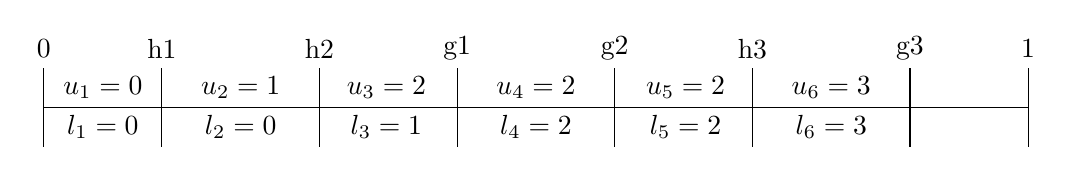
\begin{tikzpicture}
\draw (0,0) --(12.5,0);
\draw (0,-.5) --(0,.5);
\node at (0,.75) {0};
\draw (12.5,-.5) --(12.5,.5);
\node at (12.5,.75) {1};
\draw (1.5,-.5) --(1.5,.5);
\node at (1.5,.75) {h1};
\draw (5.25,-.5) --(5.25,.5);
\node at (5.25,.75) {g1};
\draw (9,-.5) --(9,.5);
\node at (9,.75) {h3};
\draw (3.5,-.5) --(3.5,.5);
\node at (3.5,.75) {h2};
\draw (7.25,-.5) --(7.25,.5);
\node at (7.25,.75) {g2};
\draw (11,-.5) --(11,.5);
\node at (11,.75) {g3};
\node at (.75,.25) {$u_{1} = 0$};
\node at (.75,-.25) {$l_{1} = 0$};
\node at (2.5,.25) {$u_{2} = 1$};
\node at (2.5,-.25) {$l_{2} = 0$};
\node at (4.35,.25) {$u_{3} = 2$};
\node at (4.35,-.25) {$l_{3} = 1$};
\node at (6.25,.25) {$u_{4} = 2$};
\node at (6.25,-.25) {$l_{4} = 2$};
\node at (8.15,.25) {$u_{5} = 2$};
\node at (8.15,-.25) {$l_{5} = 2$};
\node at (10,.25) {$u_{6} = 3$};
\node at (10,-.25) {$l_{6} = 3$};
\end{tikzpicture}
\caption{Example of how $l_{k}$ and $u_{k}$, $k = 1, ..., 2n$, depend on the relative positions of $h_{1}, ..., h_{n}$ and $g_{1}, ..., g_{n}$, for a case with n = 3. }
\end{figure}
Finally, we define
\begin{equation*}
    c_{w}^{(k)} = P_{0}(S_{k} = w \textrm{ and } l_{j} \leq S_{j} \leq u_{j} \textrm{ for } j = 1, ..., k - 1), \textrm{for } k = 1, ..., 2n \textrm{ and } w = 1, ..., n.
\end{equation*}
Our basic approach to step 1 is a recursive calculation of these $c_{w}^{(k)}$ values. Then, the global level $\alpha$ could be computed as $1 - c_{n}^{(2n)}$ in the general case. However, for the special case in which $(h_{1}, g_{1}), ..., (h_{n}, g_{n})$ are derived from equal local levels, i.e. equation (2) holds, then as a result of the symmetry in the problem, we need only calculate $c_{w}^{(k)}$ for $k = 1, ..., n+1$ instead of $k = 1, ... , 2n$. This shortcut is implemented below in the pseudocode for step 1. The algorithm calculates the probability of a valid allocation (under the null hypothesis) of points in bins by looping over each bin and making a recursive calculation.
% In this algorithm I think that I want to introduce Mary Sara's calculation. I should maybe introduce some notation before this, but I think that it's probably fine.
\begin{algorithm}[H]
\caption{Calculate Type I error $\alpha$ from proposed rejection region}
\textbf{Input:} Vector of lower bound values $(h_{1}, ..., h_{n})$, vector of upper bound values $(g_{1}, ..., g_{n})$, where we require $h_{i} < g_{i}$ for $i = 1, ..., n$.
\newline
\textit{get\_level\_from\_bounds\_two\_sided}$(h_{1}, ..., h_{n}, g_{1}, ..., g_{n})$
\begin{algorithmic}[1]
\STATE $b_{1}, ..., b_{2n} \leftarrow \textbf{sort}(h_{1}, ..., h_{n}, g_{1}, ..., g_{n})$
\STATE {$c_{0}^{(1)} \leftarrow (1 - b_{1})^{n}$}
\STATE $l_{k} \leftarrow 0$
\STATE $u_{k} \leftarrow 0$
\FOR{$k = 2, ..., n + 1$}
\IF{$b_{k - 1} \in \{h_{1}, ..., h_{n}\}$}
\STATE $u_{k} \leftarrow u_{k - 1} + 1$
\ENDIF
\IF{$b_{k} \in \{g_{1}, ..., g_{n}\}$}
\STATE $l_{k} \leftarrow l_{k - 1} + 1$
\ENDIF
\FOR{$j = l_{k}, ..., u_{k}$}
\STATE $c_{j}^{(k)} \leftarrow 0 $
\FOR{$m = l_{k - 1}, ..., min(u_{k - 1}, j)$}
\STATE $c_{j}^{(k)} \leftarrow  c_{j}^{(k)} + c_{m}^{(k - 1)} * dbinom(x = j - m, size = n-m, prob = \frac{(b_{k} - b_{k - 1})}{(1 - b_{k - 1})})$
\ENDFOR
\ENDFOR
\ENDFOR
\STATE $1 - \alpha \leftarrow 0$
\FOR{$l = l_{n}, ..., u_{n}$}
\STATE $1 - \alpha \leftarrow 1 - \alpha + \frac{c_{l}^{(n)} * c_{n - l}^{(n + 1)}}{dbinom(x = l, size = n, prob = b_{n})}$
\ENDFOR
\RETURN $\alpha$
\end{algorithmic}
\textbf{end}
\end{algorithm}
Now, we derive the algorithm. \textbf{Initialization:} (Lines 2 through 4 of Algorithm 1)
\begin{align*}
    c_{0}^{(1)} &= P_{0}(S_{1} = 0)\\
    &= P_{0}\Big(\bigcap\limits_{i=1}^{n}\{X_{i} \in (b_{1}, 1)\}\Big)\\
    &= \prod\limits_{i=1}^{n}P_{0}\Big(X_{i} \in (b_{1}, 1)\Big) &\textrm{(by independence)}\\
    &= (1 - b_{1})^{n} &\textrm{(Since each $X_{i} \sim~ U(0, 1)$ under the null)}
\end{align*}
Also, we initialize $l_{1} = 0$ and $u_{1} = 0$ because the only allowable partial sum is 0 in the first bin.
\textbf{Recursion:} (Line 15 of Algorithm 1)
\begin{flalign*}
    \indent\indent c_{j}^{(k)} &= P_{0}(S_{k} = j \textrm{ and } l_{q} \leq S_{q} \leq u_{q} \textrm{ for } q = 1, ..., k - 1)\\
    &= P_{0}\Big(\bigcup\limits_{m=l_{k- 1}}^{min(j, u_{k- 1})} \{S_{k - 1} = m \textrm{ and } N_{k} = j - m \textrm{ and } l_{q} \leq S_{q} \leq u_{q} \textrm{ for } q = 1, ..., k - 2\}\Big)\\
    &= \sum\limits_{m=l_{k- 1}}^{min(j, u_{k- 1})}P_{0}(S_{k - 1} = m \textrm{ and } N_{k} = j - m \textrm{ and } l_{q} \leq S_{q} \leq u_{q} \textrm{ for } q = 1, ..., k - 2)\\
    &= \sum\limits_{m=l_{k- 1}}^{min(j, u_{k- 1})}P_{0}(S_{k - 1} = m \textrm{ and } l_{q} \leq S_{q} \leq u_{q} \textrm{ for } q = 1, ..., k - 2)*\\
    &P_{0}(N_{k} = j - m | S_{k - 1} = m \textrm{ and } l_{q} \leq S_{q} \leq u_{q} \textrm{ for } q = 1, ..., k - 2)\\
    &= \sum\limits_{m=l_{k- 1}}^{min(j, u_{k- 1})}c_{m}^{(k - 1)} * P_{0}(N_{k} = j - m | S_{k - 1} = m)\\
    &= \sum\limits_{m=l_{k- 1}}^{min(j, u_{k- 1})}c_{m}^{(k - 1)} * P(B = j - m), \textrm{where }B \sim Binomial\left(n - m, \frac{b_{k} - b_{k - 1}}{1 - b_{k - 1}}\right),
    &&
\end{flalign*}
\newline
\indent\indent which is easily computed.
\newline
\newline
As noted above, in the general case, we could use this recursion to obtain $c_{n}^{(2n)}$, and then compute $\alpha = 1 - c_{n}^{(2n)}$. However, in the special case of equal local levels, we can use symmetry to speed the calculation by only computing the $c_{w}^{(k)}$ values for $k = 1, ..., n+1$ and $w = 1, ..., n$, and performing the calculation on line 21 of Algorithm 1, as we now demonstrate. First, we define the following values:
\begin{align*}
\Tilde{u}_{k} &=
    \begin{cases}
      0, & \text{if}\ k = 2n \\
      \sum_{i = k + 1}^{2n} \mathds{1} \big(b_{i} \in \{g_{1}, ..., g_{n}\}\big), & \text{otherwise}
    \end{cases}\\
    \Tilde{l}_{k} &=
      \sum_{i = k}^{2n} \mathds{1} \big(b_{i} \in \{h_{1}, ..., h_{n}\}\big)\\
    T_{k} &= \sum_{j = k + 1}^{2n + 1}N_{j} = n - S_{k}
\end{align*}
Now, we make the following observations:
\newline
\newline
(1) With equal local levels, $g_{i} = 1 - h_{n + 1 - i}$ for $i = 1, ..., n$ since $F_{Beta(i, n + 1 - i)}^{-1}(1 - \frac{\eta}{2})$ = $1 - F_{Beta(n + 1 - i, i)}^{-1}(\frac{\eta}{2})$.
\newline
\newline
(2) $b_{k} = 1 - b_{2n + 1 - k}$ for $k = 1, ..., 2n$ by (1). 
\newline
\newline
(3) $u_{k} = \Tilde{u}_{2n + 1 - k}$ and $l_{k} = \Tilde{l}_{2n + 1 - k}$, for $k = 1,..., 2n$ by (1) and (2).
\newline
\newline
(4) The random vector $(N_{1}, ..., N_{k})$ has the same distribution as $(N_{2n + 1}, ..., N_{2n+2-k})$ for $k = 1, ..., 2n + 1$. This follows from the fact that the vector $(X_{1}, ..., X_{n})$ has the same distribution as $(1 - X_{1}, ..., 1 - X_{n})$ (since each $X_{i}$ is independent uniform) and (2).
\newline
\newline
(5) The random vector $(S_{1}, ..., S_{k})$ has the same distribution as $(T_{2n}, ..., T_{2n + 1 - k})$ for $k = 1, ..., 2n$. This follows from (4). 
\newline
\newline
(6)
\begin{align*}
    c_{j}^{(k)} &= P_{0}(S_{k} = j \textrm{ and } l_{q} \leq S_{q} \leq u_{q} \textrm{ for } q = 1, ..., k - 1)\\
    &= P_{0}(T_{2n + 1 - k} = j \textrm{ and } \Tilde{l}_{r} \leq T_{r} \leq \Tilde{u}_{r} \textrm{ for } r = 2n + 2 - k, ..., 2n).\\
\end{align*}
This follows from (3) and (5). 
\newline
\newline
(7) Conditional on $S_{k}$, the random vector $(X_{(S_{k} + 1)}, ..., X_{(n)})$ is distributed as the order statistics of $n - S_{k}$ $U(b_{k}, 1)$ independent random variables.
\newline
\newline
(8) The random vector $(S_{1}, ..., S_{r})$ and the random vector $(T_{r}, ..., T_{n})$ are independent conditional on $S_{r}$. This follows directly from (7).
\newline
\newline
Combining the above results, we can write
\begin{equation*}
    \{X_{(i)} \in (h_{i}, g_{i}) \textrm{ for } i = 1,..., n\} = \{l_{k} \leq S_{k} \leq u_{k} \textrm{ for } k = 1, ..., 2n\}
\end{equation*}
Also, observe that for any $2 \leq r \leq 2n - 1$, we have
\begin{equation*}
    \{l_{k} \leq S_{k} \leq u_{k} \textrm{ for } k = 1, ..., 2n\} = 
\end{equation*}
\begin{equation*}
    \{l_{k} \leq S_{k} \leq u_{k} \textrm{ for } k = 1, ..., r \textrm{ and } T_{r} = n - S_{r} \textrm{ and } \Tilde{l}_{k} \leq T_{q} \leq \Tilde{u}_{k} \textrm{ for } q = r, ..., 2n\}
\end{equation*}
Thus, we can write 
\begin{align*}
    \sum_{j = l_{r}}^{u_{r}} &P(S_{r} = j \textrm{ and } l_{k} \leq S_{k} \leq u_{k} \textrm{ for } k = 1, ..., r - 1)\\
    &\cdot I(\Tilde{l}_{r} \leq n - j \leq \Tilde{u}_{r})
    \cdot P(\Tilde{l}_{q} \leq T_{q} \leq \Tilde{u}_{r} \textrm{ for } q = r + 1,..., 2n | T_{r} = n - j)\\
    &= \sum_{j = l_{r}}^{u_{r}} c_{j}^{(r)} \cdot I(\Tilde{l}_{r} \leq n - j \leq \Tilde{u}_{r}) \cdot P(\Tilde{l}_{q} \leq T_{q} \leq \Tilde{u}_{r} \textrm{ for } q = r + 1,..., 2n | T_{r} = n - j) \\
    &= \sum_{j = l_{r}}^{u_{r}} c_{j}^{(r)} \cdot I(\Tilde{l}_{r} \leq n - j \leq \Tilde{u}_{r}) \cdot \frac{P(\Tilde{l}_{q} \leq T_{q} \leq \Tilde{u}_{r} \textrm{ for } q = r + 1,..., 2n \textrm{ and } T_{r} = n - j)}{T_{r} = n - j} \\
    &= \sum_{j = l_{r}}^{u_{r}} c_{j}^{(r)} \cdot \frac{c_{n - j}^{(2n + 1 - r)}}{\binom{n}{j}b_{r}^{j}(1 - b_{r})^{n-j}}
\end{align*}
Now, if we let $r = n$ above, then we get 
\begin{equation*}
    P_{0}\Big(\bigcap\limits_{i=1}^{n} X_{(i)} \in (h_{i}, g_{i})\Big) = \sum_{j = l_{n}}^{u_{n}} c_{j}^{(n)} \cdot \frac{c_{n - j}^{(n + 1)}}{\binom{n}{j}b_{n}^{j}(1 - b_{n})^{n-j}}
\end{equation*}
which is line 21 in the psuedo-code above.
\newline
\newline
Empirically, it seems that our algorithm has computational complexity $O(n^{2})$. For a dense grid of values of $n$ between $10$ and $50,000$, the number of recursive steps required (line 15 in algorithm 1 above) scales with $n^{2}$. More precisely, it appears that the number of recursive steps required is very close to $8n^{2}$. While each recursive step itself requires calculating a binomial probability which is $O((n + 1)!)$ due to the calculation of the binomial coefficient multiplied by a quantity with powers as large as $n$, these calculations can be memoized with $O(n^{2})$ cost. Thus, these binomial probability calculations do not change the big $O$ complexity of the algorithm.
\newline
\newline
% The step below should definitely be put in an algorithm float as well. I need to make sure all of this makes sense before I finish it, but afterh this the discussion and the abstract should be relatively easy to follow through on and complete.
\textbf{Step 2:} This step is done with a simple binary search over $\eta$. We begin by setting $\eta_{upper} = \frac{-log(1 - \alpha)}{(2 * log(log(n)) * log(n))}$ since this is an upper bound on the local level as shown by Gontscharuk et al., and we set $\eta_{lower} = \frac{\alpha}{n}$, as this is the lower bound given by the Bonferroni correction. The pseudocode is shown below:
\begin{algorithm}[H]
\caption{Calculate testing bounds from global level $\alpha$ and sample size $n$}
\textbf{Input:} Local level $\alpha$, sample size $n$, tolerance $\epsilon$
\newline
\textit{get\_bounds\_two\_sided}$(\alpha, n, \epsilon)$
\begin{algorithmic}[1]
\STATE $\eta_{upper} \leftarrow \frac{-log(1 - \alpha)}{(2 * log(log(n)) * log(n))}$
\STATE $\eta_{lower} \leftarrow \frac{\alpha}{n}$
\STATE $\alpha_{mid} \leftarrow \infty$
\WHILE{$\frac{\alpha_{mid} - \alpha}{\alpha} > \epsilon$}
\STATE $\eta_{mid} \leftarrow \frac{\eta_{upper} + \eta_{lower}}{2}$
\STATE $h_{1}, ..., h_{n} \leftarrow qbeta(p = \frac{\eta_{mid}}{2}$, shape1 = c(1:n), shape2 = c(n:1))
\STATE $g_{1}, ..., g_{n} \leftarrow qbeta(p = 1 - \frac{\eta_{mid}}{2}$, shape1 = c(1:n), shape2 = c(n:1))
\STATE $\alpha_{mid} \leftarrow get\_level\_from\_bounds\_two\_sided(h_{1}, ..., h_{n}, g_{1}, ..., g_{n})$
\ENDWHILE
\RETURN $h_{1}, ..., h_{n}, g_{1}, ..., g_{n}$
\end{algorithmic}
\textbf{end}
\end{algorithm}
\section{Local Level Approximations in Large Samples}
For sufficiently large values of the number of tests $n$, it can be expedient to apply an accurate asymptotic approximation of the local level $\eta$ corresponding to global level $\alpha$ in place of exact computation. Previously, Gontscharuk and Finner showed that the asymptotic local level for global level $\alpha$ and number of tests $n$ is
\begin{equation*}
    \eta_{asymp} = \frac{log(1 - \alpha)}{2log(log(n))log(n)}
\end{equation*}
\citep{gontscharuk2017asymptotics}. However, as they note, this approximation gives poor performance for $n$ even as large as $10^{4}$. To improve this approximation, they propose to add a smaller order correction term, resulting in an approximation of the form
\begin{equation}
    \eta_{approx} = \frac{log(1 - \alpha)}{2log(log(n))log(n)}\left[1 - c_{\alpha}\frac{log(log(log(n)))}{log(log(n))}\right],
\end{equation}
where $c_{\alpha}$ is chosen empirically. For the values $\alpha = .01, .05, \textrm{ and } .1$ they chose $c_{\alpha} = 1.6, 1.3, \textrm{ and } 1.1$, respectively. To select these $c_{\alpha}$ values, the authors calculated the values of $\eta$ to high precision on a grid of values up until $n = 10,000$. To further test these approximations, we decided to calculate the values of $\eta$ with high precision on a grid of values up to $n = 500,000$ for $\alpha = .01, .05$. Based on our evaluation, we found that $c_{\alpha} = 1.3$ is satisfactory for $\alpha = .05$, but that $c_{\alpha} = 1.6$ for $\alpha = .01$ was not sufficiently accurate for our purposes (see Figure 2).
\begin{figure}
\begin{center}
    \includegraphics{images/c_alpha_1_6.png}
    \includegraphics{images/c_alpha_1_591.png}
\end{center}
\caption{Relative Error of Local Level vs. Number of Tests for $\eta_{approx}$ for $\alpha = .01$ with $c_{\alpha} = 1.6$ (top) $c_{\alpha} = 1.591$ (bottom).}
\end{figure}
This approximation begins anti-conservative for small values of $n$, becomes very accurate for values of $n$ around 2,500, and then becomes and remains substantially conservative for even very large values of $n$. 
\newline
\newline
In addition to implementing algorithms 1 and 2, which, in principle, can be applied for any $n$ and $\alpha$, our package offers a faster approximate approach specifically for $\alpha = .01 \textrm{ and } .05$. For smaller values of $n$, up to $100,000$, we have pre-calculated values of $\eta$ on a dense grid of values of $n$. If the user inputs a value of $n$ less than or equal to $100,000$, we either return back the pre-computed value of $\eta$ if $n$ happens to be a grid point, or we use linear interpolation if the value of $n$ is between grid points, which leads to a highly accurate approximation. If the user inputs a value of $n$ greater than $100,000$, we use the asymptotic approximation given in (3), but with $c_{\alpha} = 1.591 \textrm{ and } 1.3$ for $\alpha = .01 \textrm{ and } .05$, respectively. We found that $c_{\alpha} = 1.591$ led to much better performance for $\alpha = .01$ for large values of $n$, as can be seen in Figure 2. Our package also implements the approximation given in equation (3) for $\alpha = .1$ with $c_{\alpha} = 1.1$, but we did not pre-compute any grid for these values due to limited computational resources.
\section{Examples}
As noted above, the algorithm presented is only correct if all of the parameters of $F_{0}$ are known, and all $X_{1}, ..., X_{n}$ are independent. While both of these assumptions may only hold in a small number of cases, the methods above are still useful in a variety of scenarios.
\newline
\newline
One of the main advantages of the local levels method, is that it can easily be used to put testing bands onto QQplots by simply graphing each $(h_{i}, g_{i})$ interval. This allows us to examine how a dataset might deviate from some null distribution much better than simply applying a test that yields a binary conclusion. Below, we present a few examples where a QQplot is useful, and where the local levels test seems ideal for assessing deviation from a global null hypothesis.

\subsection{Examining the P-value Distribution for Testing Procedures}

% It may also make sense for me to make a comparison to the Kolmogorov-Smirnov statistic at some point. I should probably include some instructive graphs or something.
% I want to have a different paragraph to better introduce the concept
% This shouldn't be too difficult
Suppose we have devised a new testing procedure to test a null hypothesis $H_{0}$ with test statistic $T(X_{1}, ..., X_{n})$, and we wish to establish that this test has correct Type I error rate.
\newline
\newline
Typically, the verification of Type I error rate is done using the following procedure:
\newline
\newline
(1) Generate $m$ simulated datasets: $(X_{1}^{(1)}, ..., X_{n}^{(1)}), ..., (X_{1}^{(m)}, ..., X_{n}^{(m)})$ under $H_{0}$.
\newline
\newline
(2) Apply the test $T$ to each of these datasets at level $\alpha$ to yield $m$ reject / not-reject conclusions: $c_{1}, ..., c_{m}$, where $c_{i} = 1$ if $H_{0}$ is rejected and $0$ otherwise.
\newline
\newline
(3) Conduct a test to confirm that the mean of $c_{1}, ..., c_{m}$ is $\alpha$.
\newline
\newline
While the above procedure provides reliable information about the Type I error calibration for one level of $\alpha$, it provides little information about the global calibration of p-values. Instead, we suggest the following procedure:
\newline
\newline
(1) As above.
\newline
\newline
(2) Apply the test $T$ to each of these datasets to yield $m$ p-values: $p_{1}, ..., p_{m}$.
\newline
\newline
(3) Apply the local levels procedure to test if $p_{1}, ..., p_{m} \distras{iid} U(0, 1)$.
% It seems to me that this would be an opportune time to make a comparison to the KS-test, but I'm not totally sure.
% I should maybe put some graphs here as well.
\newline
\newline
This allows us to easily visualize the global calibration of the p-values with just one graph and diagnose any issues if they exist. In Step 3, one could use many different testing bands. However, in the calibration of p-values, we typically don't have the expectation that our p-values would be more likely to deviate from uniform in some regions than others, and so it makes sense to use the local levels test because it is agnostic to the alternative distribution. Moreover, since it is generally most concerning if p-values are not calibrated in the lower tail of the distribution, the local levels test is preferable to the standard KS test because it is much more sensitive in the tails (Aldor-Noiman 2013).

\subsubsection{Chi-Square Test for Independence in a \texorpdfstring{$2 \times 2$}{2 X 2} Table}



\bibliography{refs}
\end{document}
